\documentclass[12pt,a4paper,oneside]{article}
\usepackage[a4paper,left=4cm,right=3cm,top=3cm,bottom=3cm]{geometry}
\usepackage{color}
\usepackage[bahasai]{babel}
\usepackage{graphicx}
\usepackage{listings}
\usepackage{xcolor}
\usepackage{float}
\usepackage{indentfirst}
\usepackage{titlesec}
\usepackage{hyperref}
\renewcommand*{\thesection}{\Alph{section}.}
\renewcommand*{\thesubsection}{\arabic{subsection}.}
\renewcommand*{\thesubsubsection}{\roman{subsubsection}.}
\titleformat*{\section}{\fontsize{12}{15}\bfseries}
\titleformat*{\subsection}{\fontsize{12}{15}\bfseries}
\lstset{language=[Sharp]C,
	numbers=left,
	stepnumber=1,
	numberstyle=\ttfamily,
	basicstyle=\ttfamily\scriptsize,
	keywordstyle=\color{blue}\ttfamily,
	stringstyle=\color{red}\ttfamily,
	commentstyle=\color{gray}\ttfamily,
	morecomment=[l][\color{magenta}]{\#},
    breaklines=true,
	frame = single, 
    %postbreak=\mbox{\textcolor{red}{$\hookrightarrow$}\space}
}


\title{\large{\textbf{LAPORAN TUGAS AKHIR}\linebreak \textbf{VISUALISASI DIJKSTRA}\linebreak}}
\date{}
\begin{document}
\begin{titlepage}
\maketitle
\begin{center}

\includegraphics[width=5cm,height=5cm]{images/logo-its.png}
\end{center}
\begin{center}
\end{center}
\vspace{0.5 cm}
\begin{center}
% create tabular 2 column 3 row
\begin{tabular}{l l}
Nama & : \author{Akhmad Thoriq Afif}\\
NRP & : 5024201028\\
Kelas & : Struktur Data B\\
\end{tabular}
\end{center}
\vspace{0.5 cm}
\begin{center}
Untuk Memenuhi Tugas Akhir Struktur Data dan Algoritma \\
Dosen Pengampu: Dr. Eko Mulyanto Yuniarno, ST., MT. \linebreak
\mbox{}
\vfill
Program Studi Teknik Komputer \\
\textit {Institut Teknologi Sepuluh Nopember}
\linebreak
Surabaya 2021 \linebreak
\end{center}
\end{titlepage}
\newpage
\section{DESKRIPSI PROGRAM}
Program ini merupakan program visualisasi dari algoritma Dijkstra. Program ini dibuat menggunakan bahasa C\#. Untuk interface pada program ini berbentuk editor, sehingga pengguna dapat menambahkan node, menghapus node, menyambungkan 2 node, memindahkan node dengan menggunakan mouse layaknya editor foto. Di bawah ini merupakan tampilan dari program ini. \par
\begin{figure}[H]
	\centering
	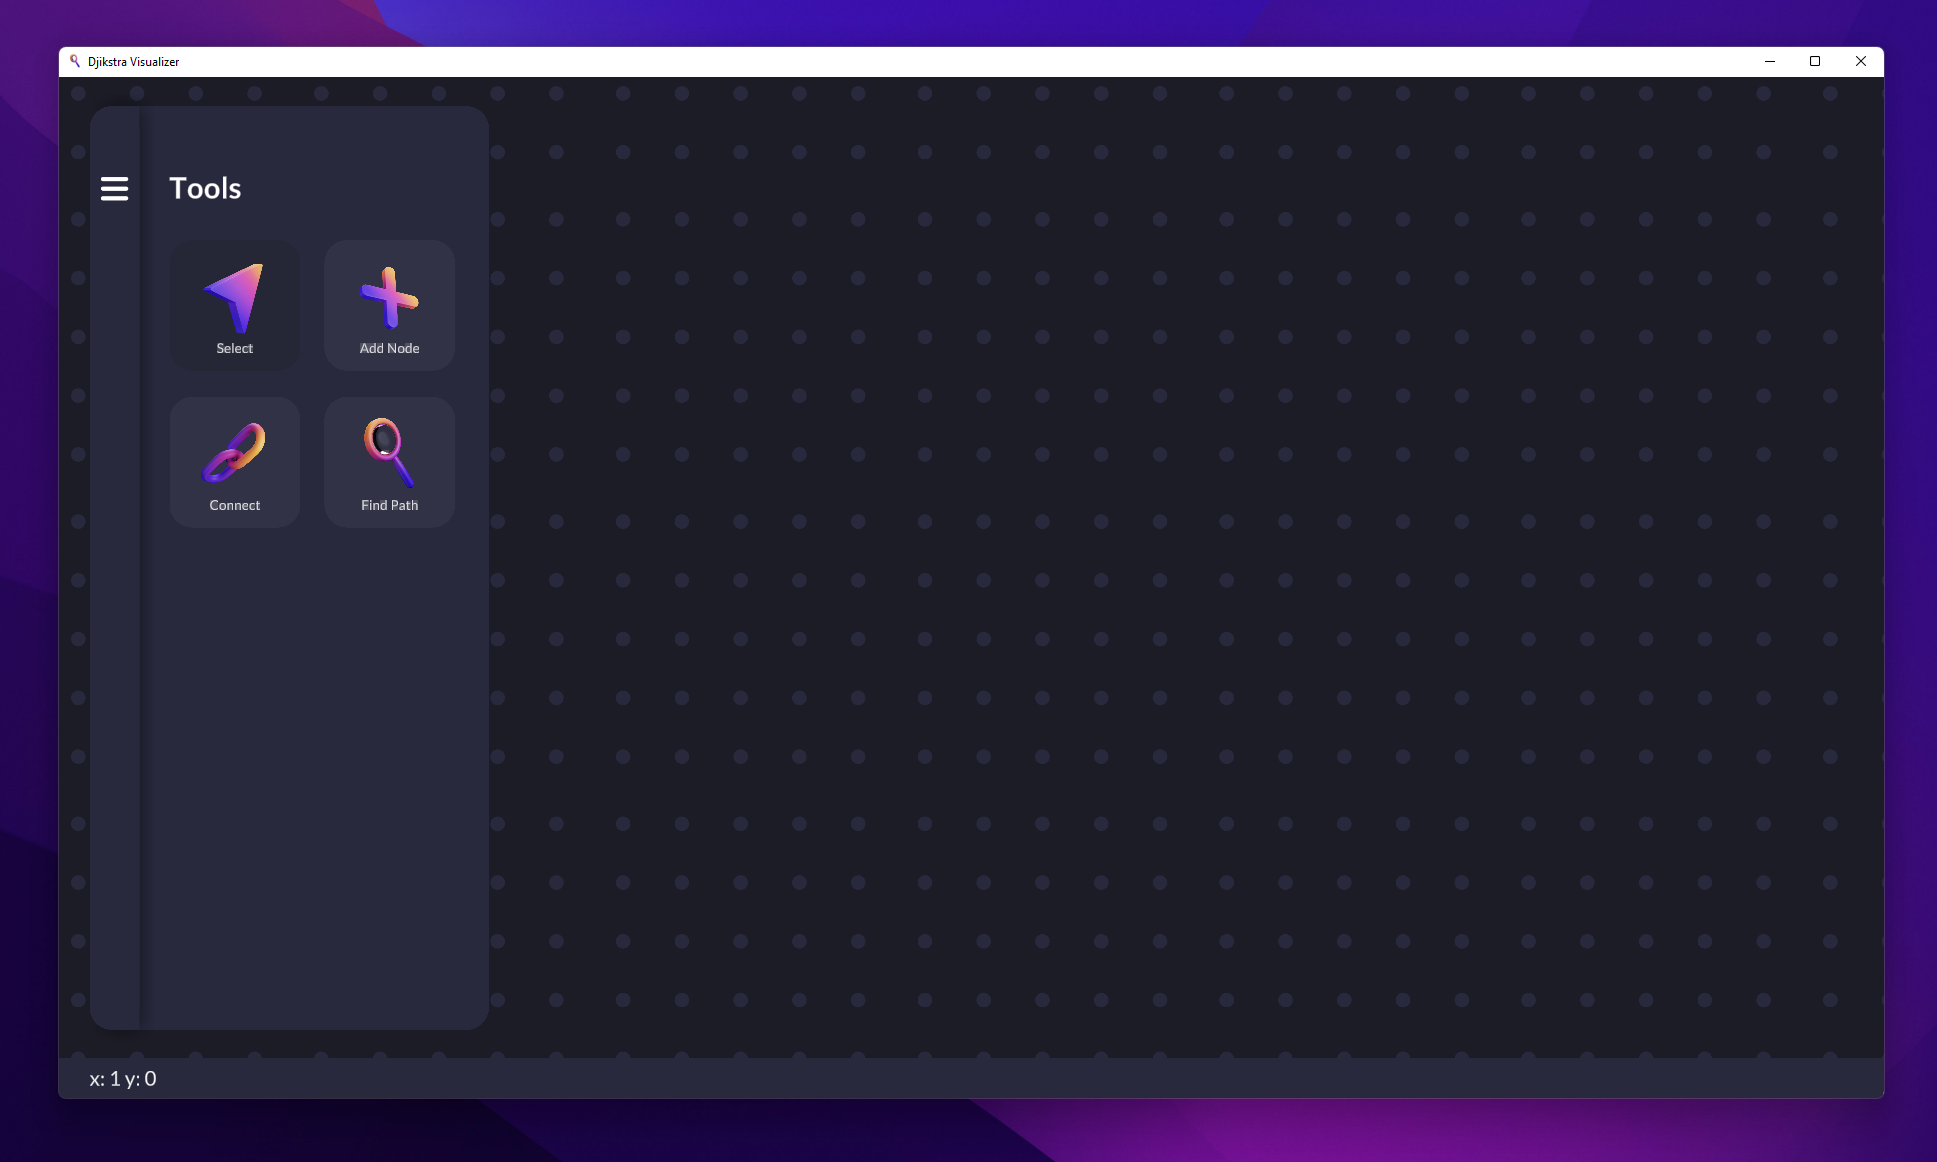
\includegraphics[width=0.8\textwidth]{images/tampilan-awal.png}
	\caption{Tampilan Awal Program}
\end{figure}
\begin{figure}[H]
	\centering
	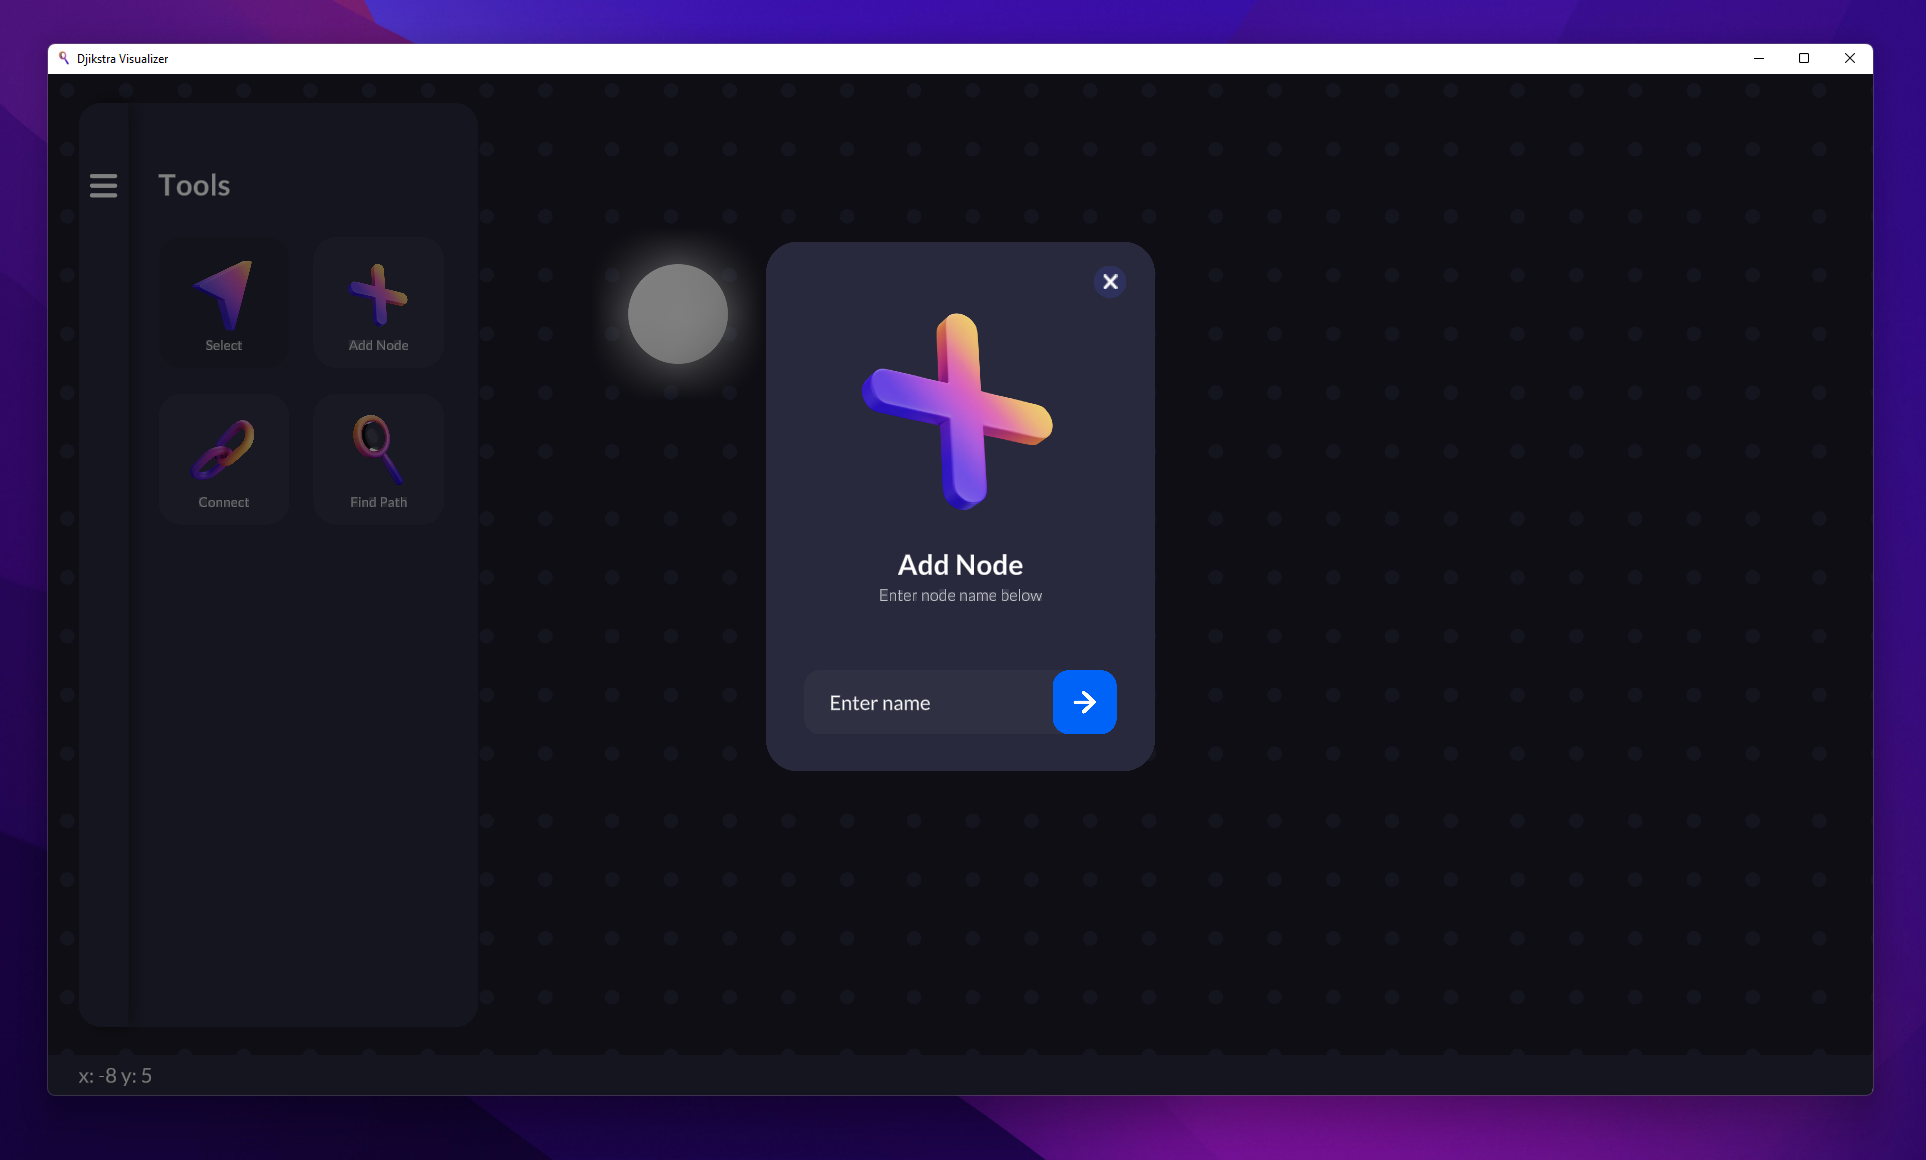
\includegraphics[width=0.8\textwidth]{images/add-node.png}
	\caption{Tampilan ketika menambahkan node}
\end{figure}
\begin{figure}[H]
	\centering
	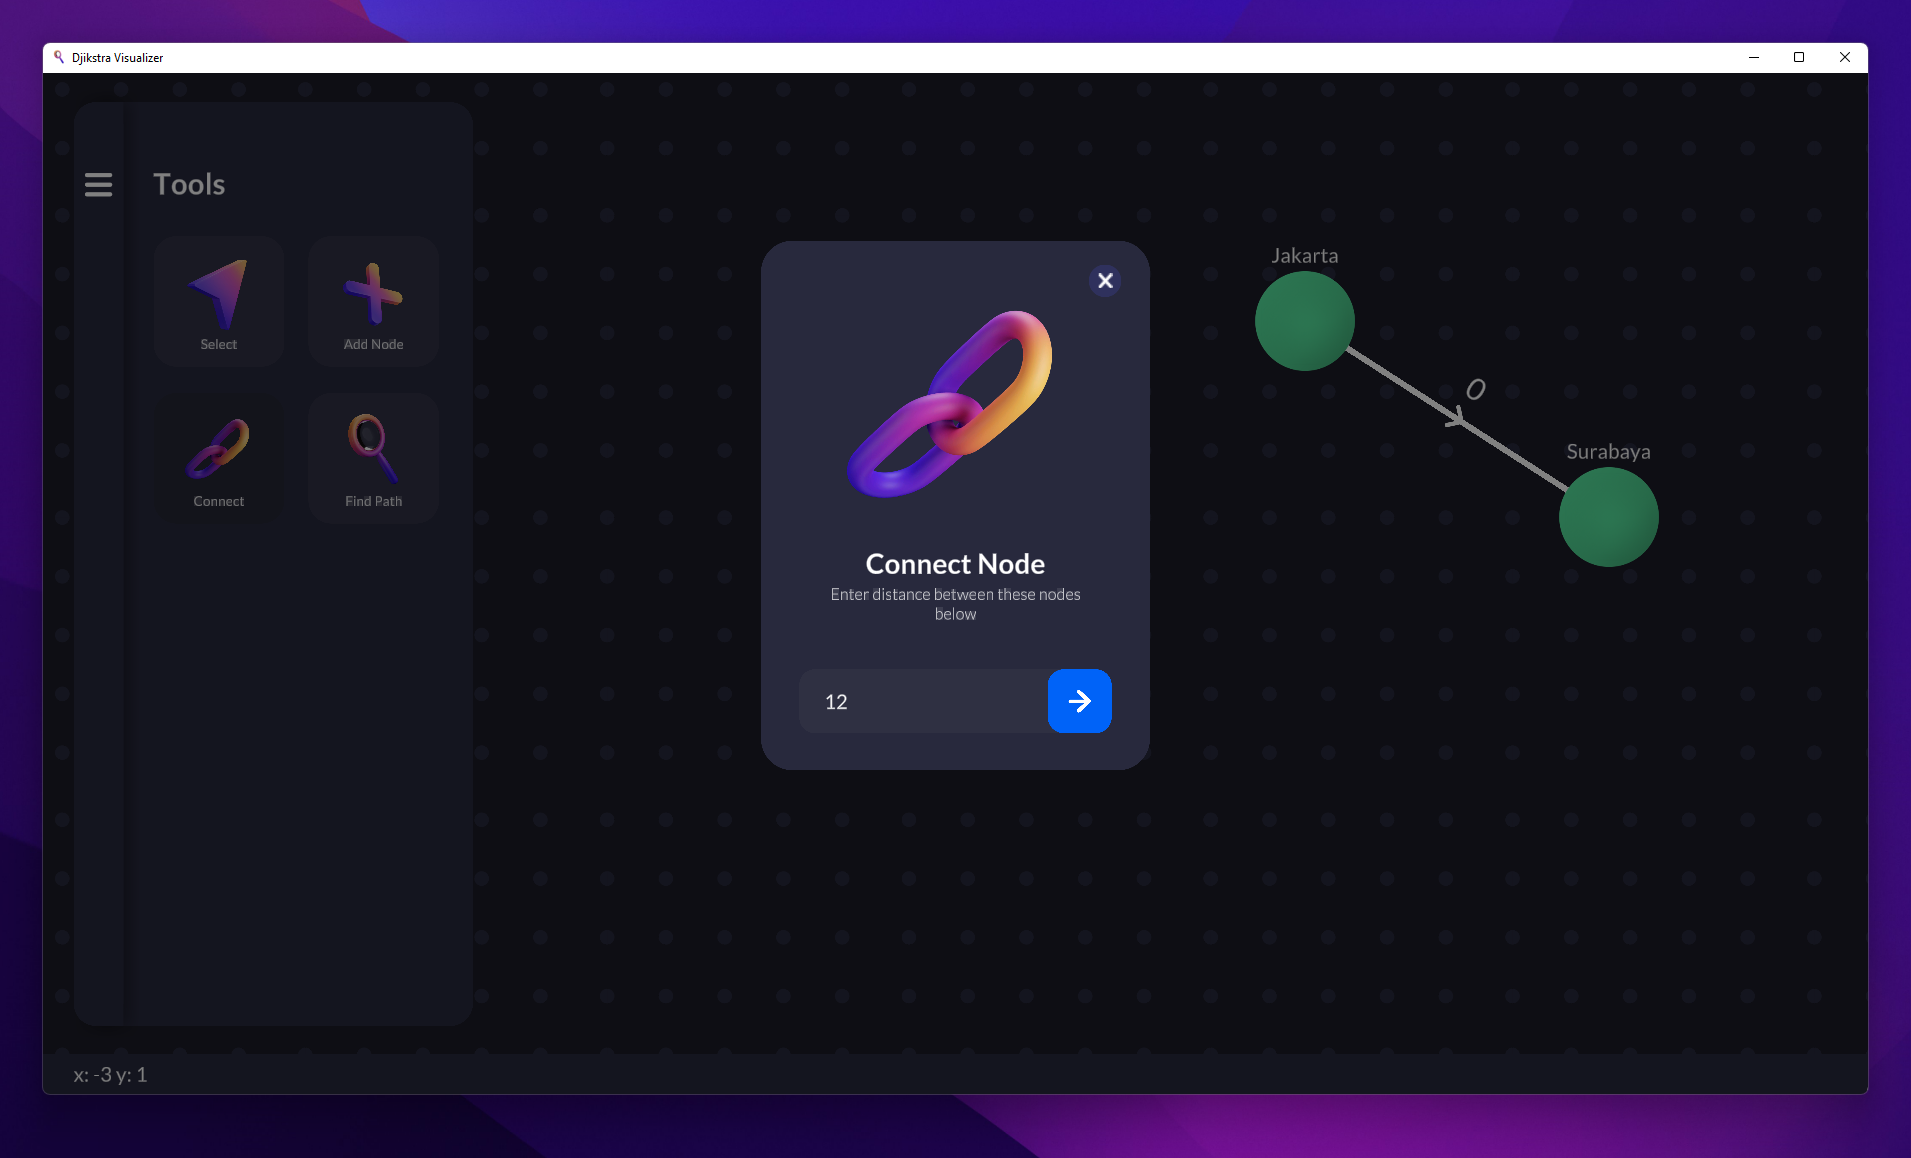
\includegraphics[width=0.8\textwidth]{images/connect-node.png}
	\caption{Tampilan ketika menghubungkan node}
\end{figure}
\begin{figure}[H]
	\centering
	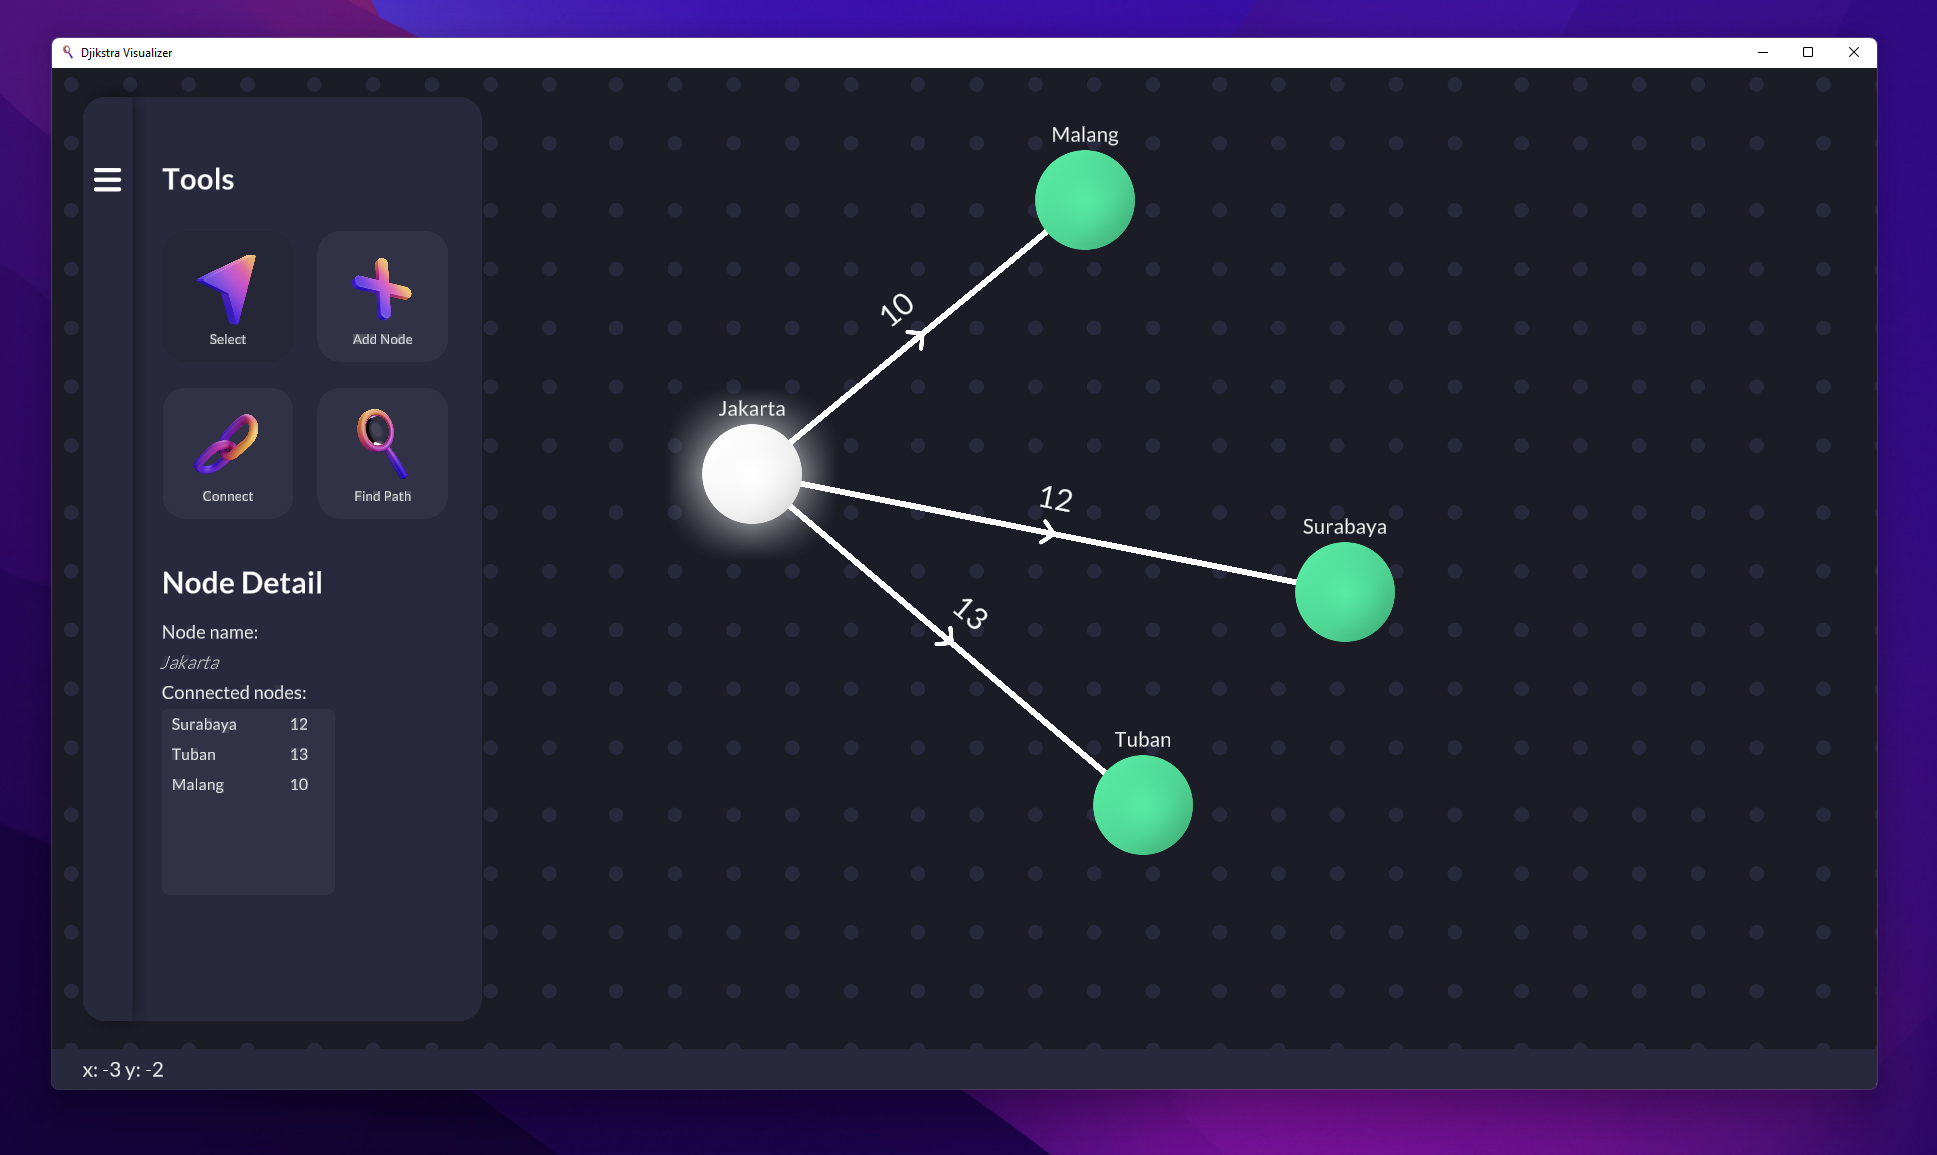
\includegraphics[width=0.8\textwidth]{images/node-detail.png}
	\caption{Tampilan node detail}
\end{figure}
\begin{figure}[H]
	\centering
	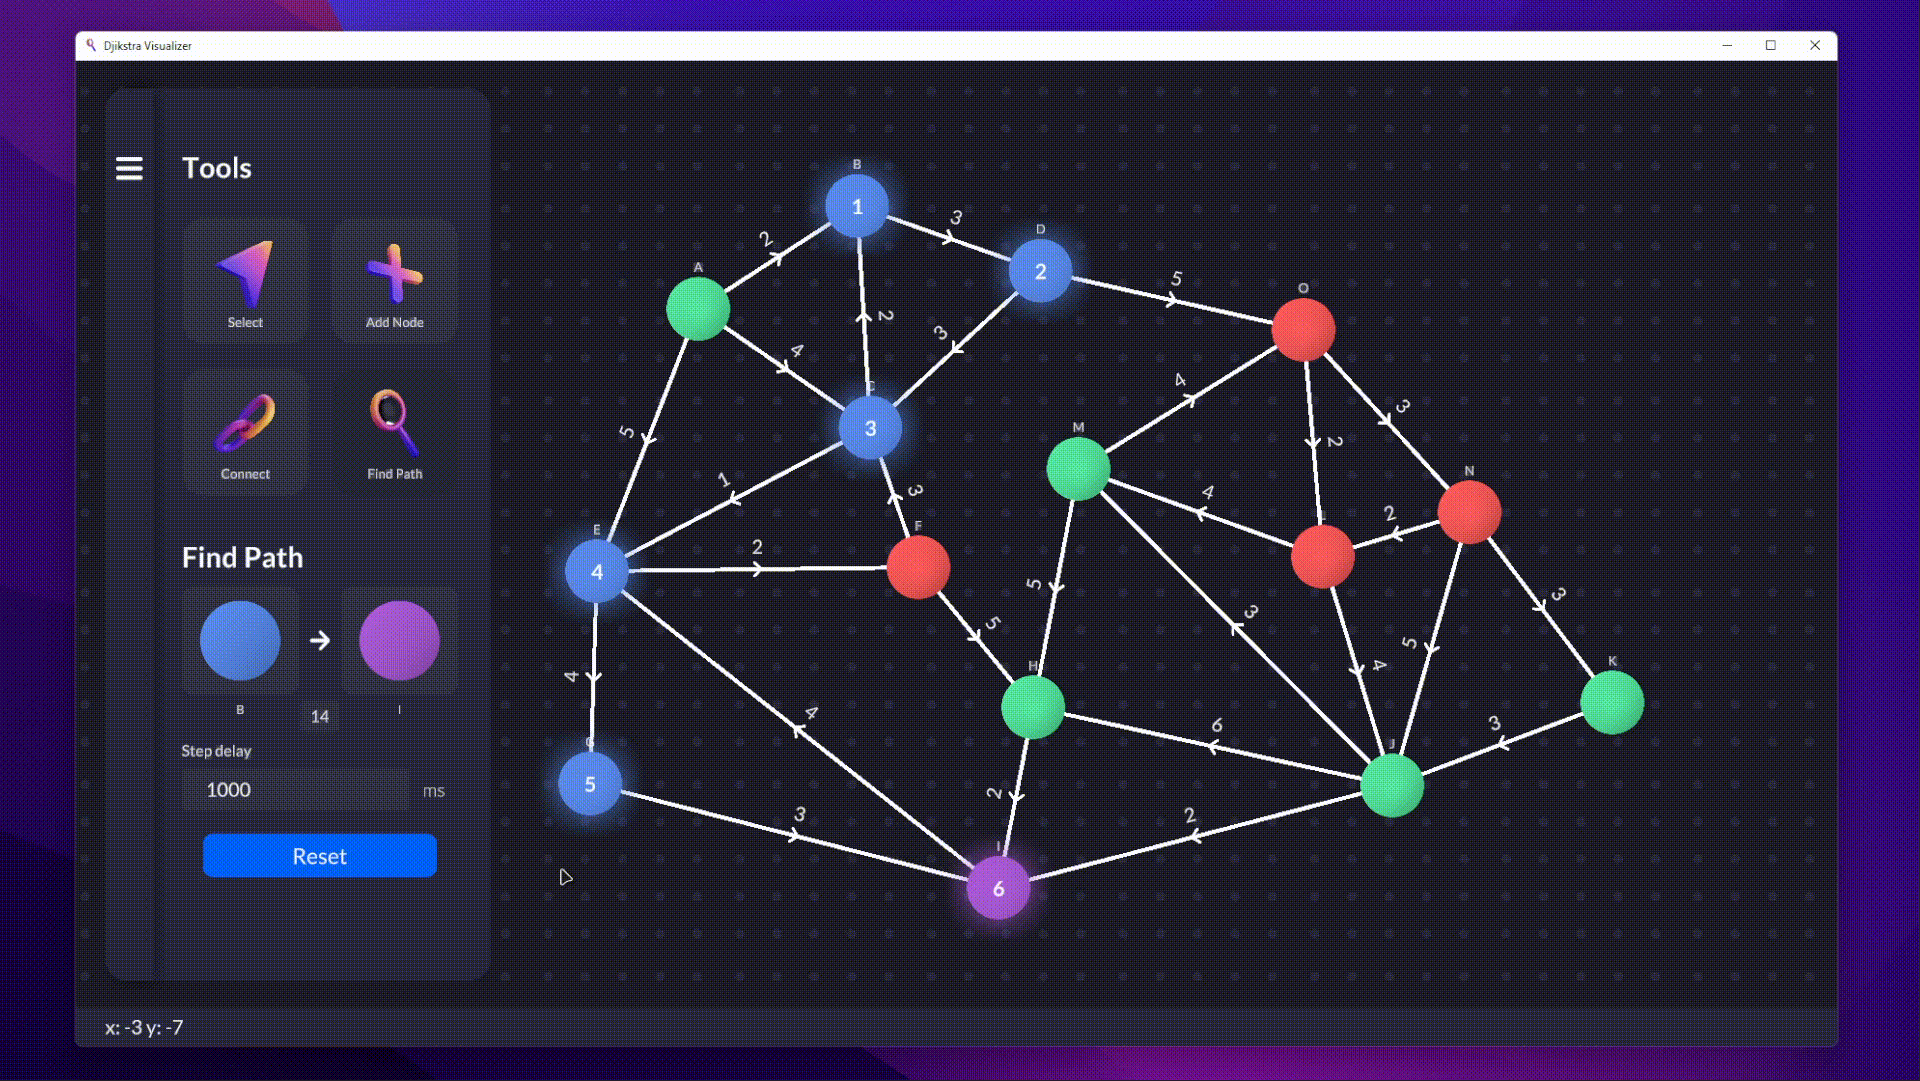
\includegraphics[width=0.8\textwidth]{images/find-path.png}
	\caption{Visualisasi path finding}
\end{figure}
Pada bagian kiri program terdapat toolbox yang berisikan tombol select, add node, connect, dan find path. Sedangkan pada bagian kiri bawah, terdapat koordinat letak mouse. Tombol select sendiri berfungsi untuk memindah node dan memilih node dengan cara double click pada node yang akan dipilih. Ketika node terpilih, maka akan muncul node detail pada bagian bawah toolbox (Gambar 2). Selain itu pengguna juga dapat menghapus node tersebut dengan menekan tombol delete. Untuk menambahkan node baru dapat digunakan tombol add node, ketika node diletakkan maka akan muncul dialog seperti pada Gambar 2. Pada dialog tersebut pengguna diminta untuk memasukkan nama dari node tersebut. Tombol connect berfungsi untuk menghubungkan dua node. Proses penyambungan dilakukan dengan cara mendrag node awal ke node tujuan. Setelah dihubungkan maka akan muncul dialog untuk memasukkan jarak antar kedua node tersebut (Gambar 3). Tombol find path digunakan untuk mencari jarak terpendek dari dua node. Hasil dari pencarian dapat dilihat pada Gambar 4 \par

\newpage
\section{LISTING PROGRAM}
\par Pada program ini terdapat beberapa class yang memiliki fungsi masing-masing. Di bawah ini merupakan listing dari class-class tersebut.
\subsection{Class AppSettings}
\lstinputlisting[label={AppSettings},caption={AppSettings.cs}, language={[Sharp]C}]{scripts/AppSettings.cs}
\subsection{Class Utils}
\lstinputlisting[label={Utils},caption={Utils.cs}, language={[Sharp]C}]{scripts/Utils.cs}
\subsection{Class States}
\lstinputlisting[label={States},caption={States.cs}, language={[Sharp]C}]{scripts/States.cs}
\subsection{Class ObjectFactory}
\lstinputlisting[label={ObjectFactory},caption={ObjectFactory.cs}, language={[Sharp]C}]{scripts/ObjectFactory.cs}
\subsection{Class CameraController}
\lstinputlisting[label={CameraController},caption={CameraController.cs}, language={[Sharp]C}]{scripts/CameraController.cs}
\subsection{Class AppManager}
\lstinputlisting[label={AppManager},caption={AppManager.cs}, language={[Sharp]C}]{scripts/AppManager.cs}
\subsection{Class CursorStateManager}
\lstinputlisting[label={CursorStateManager},caption={CursorStateManager.cs}, language={[Sharp]C}]{scripts/CursorStateManager.cs}
\subsection{Class GraphManager}
\lstinputlisting[label={GraphManager},caption={GraphManager.cs}, language={[Sharp]C}]{scripts/GraphManager.cs}
\subsection{Class PathfindingManager}
\lstinputlisting[label={PathfindingManager},caption={PathfindingManager.cs}, language={[Sharp]C}]{scripts/PathfindingManager.cs}
\subsection{Class Djikstra}
\lstinputlisting[label={Djikstra},caption={Djikstra.cs}, language={[Sharp]C}]{scripts/Djikstra.cs}
\subsection{Class Node}
\lstinputlisting[label={Node},caption={Node.cs}, language={[Sharp]C}]{scripts/Node.cs}
\subsection{Class NodeState}
\lstinputlisting[label={NodeState},caption={NodeState.cs}, language={[Sharp]C}]{scripts/NodeState.cs}
\subsection{Class NodeController}
\lstinputlisting[label={NodeController},caption={NodeController.cs}, language={[Sharp]C}]{scripts/NodeController.cs}
\subsection{Class NodeTextController}
\lstinputlisting[label={NodeTextController},caption={NodeTextController.cs}, language={[Sharp]C}]{scripts/NodeTextController.cs}
\subsection{Class EdgeData}
\lstinputlisting[label={EdgeData},caption={EdgeData.cs}, language={[Sharp]C}]{scripts/EdgeData.cs}
\subsection{Class EdgeLineController}
\lstinputlisting[label={EdgeLineController},caption={EdgeLineController.cs}, language={[Sharp]C}]{scripts/EdgeLineController.cs}
\subsection{Class EdgeLineChildController}
\lstinputlisting[label={EdgeLineChildController},caption={EdgeLineChildController.cs}, language={[Sharp]C}]{scripts/EdgeLineChildController.cs}
\subsection{Class GUIManager}
\lstinputlisting[label={GUIManager},caption={GUIManager.cs}, language={[Sharp]C}]{scripts/GUIManager.cs}
\subsection{Class ToastGUI}
\lstinputlisting[label={ToastGUI},caption={ToastGUI.cs}, language={[Sharp]C}]{scripts/ToastGUI.cs}
\subsection{Class DialogGUI}
\lstinputlisting[label={DialogGUI},caption={DialogGUI.cs}, language={[Sharp]C}]{scripts/DialogGUI.cs}
\subsection{Class BlackBlockerGUI}
\lstinputlisting[label={BlackBlockerGUI},caption={BlackBlockerGUI.cs}, language={[Sharp]C}]{scripts/BlackBlockerGUI.cs}
\subsection{Class ToolsBoxGUI}
\lstinputlisting[label={ToolsBoxGUI},caption={ToolsBoxGUI.cs}, language={[Sharp]C}]{scripts/ToolsBoxGUI.cs}
\subsection{Class ToolsButtonGUI}
\lstinputlisting[label={ToolsButtonGUI},caption={ToolsButtonGUI.cs}, language={[Sharp]C}]{scripts/ToolsButtonGUI.cs}
\subsection{Class CoordinateInfoGUI}
\lstinputlisting[label={CoordinateInfoGUI},caption={CoordinateInfoGUI.cs}, language={[Sharp]C}]{scripts/CoordinateInfoGUI.cs}
\newpage
\section{PENJELASAN PROGRAM}
\subsection{Class AppSettings}
Class ini berisikan setting dari program ini.
\begin{itemize}
	\item \textbf{Line 21} : Berfungsi untuk membatasi framerate dari aplikasi. Pada aplikasi ini framerate dibatasi sebesar 60fps. Pembatasan ini dilakukan untuk mengurangi CPU maupun GPU load.
\end{itemize}
\subsection{Class Utils}
Class ini berisikan fungsi-fungsi umum yang digunakan pada program ini.
\begin{itemize}
	\item \textbf{Line 5-11} : Fungsi getMouseWorldPosition() digunakan untuk mendapatkan posisi mouse yang relatif pada posisi world. Pada fungsi ini dilakukan pengubahan dari posisi mouse yang relatif pada posisi screen menjadi posisi mouse yang relatif pada posisi world dengan menggunakan fungsi ScreenWorldPoint();
\end{itemize}
\subsection{Class States}
Class ini berisikan class enum yang digunakan sebagai penanda pada aplikasi ini. Pada class ini terdapat beberapa enum class yaitu CursorState, ToolsType, dan PFStates. CursorStates digunakan untuk menandai state dari cursor. ToolsType digunakan pada class ToolsButtonGUI untuk menentukan tipe tool dari tombol tersebut. PFStates digunakan untuk menandai state dari Pathfinding, apakah state tersebut dalam keadaan Idle, Running, Stopped atau Finished.
\subsection{Class ObjectFactory}
Class ini berisikan method-method yang berfungsi dalam pembuatan objek baru, seperti pembuatan objek EdgeLine dan Node.
\begin{itemize}
	\item \textbf{Line 24-37} : Fungsi createEdgeLine() digunakan untuk membuat objek EdgeLine. Pada fungsi ini dilakukan pembuatan objek EdgeLine dengan menggunakan fungsi Instantiate(). Peletakan objek ini didasarkan pada posisi yang diinput pada parameter fungsi. Pada program ini parameter yang diinputkan adalah posisi node yang sedang dipilih.
	\item \textbf{Line 39-41} : Fungsi createNode() digunakan untuk membuat objek Node. Sama halnya dengan fungsi createEdgeLine(), pembuatan objek dilakukan dengan menggunakan fungsi Instantiate().
\end{itemize}
\subsection{Class CameraController}
Class ini berfungsi untuk mengontrol kamera, seperti mengatur posisi kamera maupun zoom.
\begin{itemize}
	\item \textbf{Line 5-20} : Dilakukan penginisiasian properti yang digunakan pada class ini.
	\item \textbf{Line 25-30} : Pada baris ini dilakukan pemindahan posisi kamera. Pemindahan posisi dilakukan ketika tombol tengah mouse ditekan pada frame sebelumnya. Jarak pemindahan dihitung dari posisi kursor sekarang dikurangi posisi kursor ketika tombol tengah mouse ditekan.
	\item \textbf{Line 32-38} : Perhitungan target zoom kamera. Perhitungan didasarkan pada nilai return dari InputGetAxis(). Jika nilai return dari fungsi tersebut bernilai negatif maka dilakukan penambahan zoom. Jika nilai return dari fungsi tersebut bernilai positif maka dilakukan pengurangan zoom. Penambahan atau pengurangan zoom ini dibatasi dengan fungsi Clamp(). Pada baris ini hanya dilakukan perhitungannya saja, untuk eksekusinya akan dilakukan pada kode baris ke 43.
	\item \textbf{Line 41} : Pengambilan posisi kursor relatif terhadap world. Nilai ini nantinya akan digunakan untuk menggeser titik tengah kamera menuju posisi kursor ketika melakukan zoom.
	\item \textbf{Line 43} : Berfungsi untuk melakukan pengurangan atau penambahan pada orthographicSize kamera untuk memberikan efek zoom. Digunakan fungsi Lerp() agar pergerakan zoom menjadi lebih halus.
	\item \textbf{Line 45-49} : Berfungsi untuk menampilkan Toast yang berisikan informasi skala zoom kamera.
	\item \textbf{Line 51-56} : Berfungsi untuk menggeser kamera ke titik tengah kursor.
	\item \textbf{Line 59-62} : Berfungsi untuk mengambil posisi dari kursor. Nilai ini digunakan untuk menggeser posisi kamera.
\end{itemize}
\subsection{Class AppManager}

\begin{itemize}
	\item \textbf{Line 9-17} : Penginisiasian properti yang akan digunakan pada class ini.
	\item \textbf{Line 18-38} : Fungsi getter dan setter untuk properti mselectedNodeProperty. Ketika fungsi setter dipanggil/ketika nilai dari properti mselectedNodeProperty diubah maka akan dilakukan pengubahan nilai monSelectedChanged menjadi true. monSeletedChanged ini akan digunakan pada class ToolsBoxGUI untuk mengupdate tampilan NodeDetail.
	\item \textbf{Line 57-58} : Digunakan untuk mensetting double click. Digunakan nilai 250 milisecond sebagai batas waktu double click dan fungsi singleClick() ketika nilai mdoubleClickTimer melebihi nilai 250 milisecond.
	\item \textbf{Line 64-115} : Digunakan pada saat state dari cursor bernilai Add. Baris ini berfungsi untuk menambahkan node baru. Ketika mnewNode bernilai null maka akan dibuat node baru. Jika mnewNode tidak bernilai null alias sudah dibuat maka node tersebut akan bergerak mengikuti kursor. Pada baris 82-87 pengguna dapat membatalkan penambahan node dengan menekan delete. Ketika pengguna menekan tombol kiri mouse maka akan muncul dialog untuk memasukkan nama dari node tersebut. Dialog ini berasal dari pemanggilan showDialog() yang berada pada class GUIManager. Diinputkan parameter callback function yang akan dipanggil ketika tombol OK pada dialog ditekan.
	\item \textbf{Line 118-152} : Berfungsi untuk memilih node. Pemilihan node dilakukan ketika cursor state bernilai Select dan pengguna melakukan double click pada node. Node yang dipilih akan disimpan pada mselectedNode.
	\item \textbf{Line 153-182} : Berfungsi untuk emmilih node start dan node end. Pemiliian node dilakukan ketika cursor state bernilai FindPath. Pemilihan node start dan node end cukup dengan melakukan single click.
	\item \textbf{Line 184-193} : Berfungsi untuk menghapus node yang sedang dipilih/berada dalam property mselectedNode.
	\item \textbf{Line 197-200} : Dipanggil ketika nilai mmouseClickTimer melebihi batas yaitu 250 milisecond. Fungsi ini akan menstop mmouseClickTimer() sehingga nilainya akan kembali ke 0.
	\item \textbf{Line 202-220} : Merupakan fungsi untuk melakukan double click. Paremeter pertama pada fungsi ini adalah fungsi void yang akan dijalankan ketika singleClick terjadi. Parameter kedua adalah fungsi void yang akan dijalankan ketika doubleClick terjadi. sedangkan parameter terakhir adalah index button yang ditekan.
\end{itemize}
\subsection{Class CursorStateManager}
Class ini berfungsi untuk menyimpan state dari cursor.
\subsection{Class GraphManager}
Class ini berisikan property yang menyimpan data graph dan method-method yang digunakan untuk mengubah data graph.
\begin{itemize}
	\item \textbf{Line 10} : Penginisiasian graphContainer berbentuk Dctionary yang digunakan untuk menyimpan Node beserta EdgeData-nya. Key dari graphContainer ini adalah objek Node dan Valuenya berupa tuple yang keduannya berisikan list objek EdgeData. Untuk tuple Item 1 merupakan EdgeData yang masuk kedalam Node. Sedangkan, Item 2 merupakan EdgeData yang keluar dari Node.
	\item \textbf{Line 27-41} : Fungsi addEdgeLine() berfungsi untuk menambahkan objek edgeLine kedalam graphContainer. Fungsi ini dipanggil ketika mengoneksikan dua Node.
	\item \textbf{Line 43-72} : Fungsi deleteNode() berfungsi untuk menghapus node dan objek EdgeLine.
	\item \textbf{Line 74-82} : Fungsi getEdgeList() berfungsi untuk Value dari Key yang dimasukkan sebagai parameter.   
\end{itemize}
\subsection{Class PathfindingManager}
Class ini berfungsi untuk mengatur jalannya proses pathfinding.
\begin{itemize}
	\item \textbf{Line 25-28} : Fungsi registertask() dipanggil ketika tombol Start yang berada di panel toolsbox ditekan. Fungsi ini akan memasukkan IEnumerator yang mana pada program ini adalah fungsi dijkstra kedalam mCoroutine. Penyimpanan ini memudahkan ketika menstop Coroutine.
	\item \textbf{Line 38-34} : Sama dengan fungsi registertas(), fungsi start() dipanggil ketika tombol Start yang berada di panel toolsbox ditekan. Fungsi ini akan memulai Coroutine dan mengubah state menjadi Running. Penggunaan Coroutine ini bertujuan agar proses pathfinding dapat berjalan secara asynchronous dan tidak memblok jalanya program karena dalam fungsi dijkstra dilakukan beberapa kali delay. Delay ini bertujuan agar visualisasi lebih terlihat.
	\item \textbf{Line 36-39} : Fungsi stop() berfungsi untuk menggentinkan proses pathdinging. Fungsi ini mengubah state menjadi Stopped.
\end{itemize}
\subsection{Class Djikstra}
Class ini berisikan fungsi-fungsi static yang digunakan dalam melakukan pathfinding menggunakan metode Dijkstra. Pada fungsi pencarian pathfinding menggunakan IEnumerator, ini bertujuan agar sewaktu-waktu fungsi dapat di-"pause" sehingga tidak memblok jalanya program. Pda fungsi findShortestPath() dibutuhkan parameter berupa graphlist, node start, node end, dan step delay.
\begin{itemize}
	\item \textbf{Line 7-12} : Pada baris ini dilakukan pengecekan apakah node start terhubung dengan node lain jika tidak maka akan ditampilkan toast dengan informasi bahwa "jalur tidak dapat ditemukan" dan pencarian dibatalkan dengan melakukan yield break. Jika tidak maka pencarian akan dilanjutkan.
	\item \textbf{Line 15-17} : Dilakukan penginisiasian container yang dibutuhkan yaitu distance list yang digunakan untuk menyimpan jarak, previouslist yang digunakan untuk menyimpan node sebelumnya, dan unvisitedlist yang digunakan untuk menyimpan node yang belum dikunjungi. 
	\item \textbf{Line 19-23} : Pada distanceList dilakukan penginputan node sebagai key dan maxValue dari float sebagai Value. Pada unvisitedList dilakukan penginputan semua node. Beigtupun juga dengan previousList.
	\item \textbf{Line 25} : pada distanceList, untuk node yang merupakan start node nilai valuenya diubah menjadi 0. Sehingga node yang akan dikunjungi paling awal adalah node start.
	\item \textbf{Line 28-32} : Pada baris ini dilakukan pengambilan node dengan distance terkecil yang ada pada unvisitedList. Pengabilan tersebut dilakukan dengan memanggil fungsi GetNodeWithLowestDistance(). Selanjutnya Node yang terpilih dihapus dari unvisitedList. Kemudian warna node diubah menjadi kuning dengan memanggil setAccessed. Ini memberikan visualisasi bahwa node sedang diaccess.
	\item \textbf{Line 34} : Dilakukan yield return pada baris ini dengan delay sebesar stepDelay yang telah diinput. Ini bertujuan untuk memberikan jarak waktu visualisasi.
	\item \textbf{Line 36-72} : Pada baris ini dilakukan pengecekan jika currentNode adalah node end maka jalur akan disusun. Penyusunan jalur dilakukan dengan memasukkan nodePrevious dari node end sampai ke node start ke dalam container berbentuk stack. Digunakan container stack agar susunan menjadi terbalik, sehingga jalur dimulai dari node start. Setelah disusun, node yang terdapat pada stack akan diubah warnanya menjadi biru, diberi efek glow, dan ditampilkan angka step tiap nodenya.
	\item \textbf{Line 74-80} : Pada baris ini dilakukan transversal pada list node yang terkoneksi dengan currentNode. Untuk setiap node yang terkoneksi jaraknya ditambahkan dengan jarak currentNode yang terdapat pada distanceList. Hasil penambhan ini disimpan kedalam newDistance. Kemudian newDistance dibandingkan dengan jarak neighbour yang terdapat pada distanceList. Jika newDistance lebih kecil maka jarak neighbour pada distanceList diubah menjadi newDistance dan previouslist[neighbour] diubah menjadi currentNode.
	\item \textbf{Line 82} : Dilakukan pengubahan warna currentnode menjadi merah dengan memanggil setVisisted. Hal ini untuk memvisualisasikan bahwa node telah dikunjungi.
	\item \textbf{Line 92-104} : Fungsi GetNodeWithLowestDistance() berfungsi untuk mendapatkan node dengan jarak terkecil yang ada pada unvisitedList dengan perbandingan jaraknya berdasarkan distancelist. 
\end{itemize}
\subsection{Class Node}
Class ini bersikan property mConnectedNodes berbentuk Dictionary dengan Key Node dan Value EdgeData. mConnectedNodes ini digunakan untuk menyimpan node-node yang terhubung.
\begin{itemize}
	\item \textbf{Line 10-18} : Merupakan getter setter dari mnodeNameProperty. Saat melalukan perubahan nilai mnodeNameProperty akan dilakukan pemanggilan updateNodeName() yang berada pada class NodeTextController, ini bertujuan untuk mengubah tampilan nama node.
	\item \textbf{Line 26-36} : Fungsi connect() digunakan untuk melakukan koneksi antara dua node.
	\item \textbf{Line 38-45} : Fungsi allowConnect() digunakan untuk mengecek apakah node yang dituju dapat dihubungkan atau tidak dengan cara mengecek apakah dalam mConnectedNodes sudah ada node yang sama dengan node yang dituju. Hal ini untuk menghindari koneksi antar node yang sama.
	\item \textbf{Line 49-58} : Fungsi checkTwoWayConnection() berfungsi untuk mengecek apakah node yang dituju sudah terhubung dengan node yang sedang dihubungkan. Fungsi ini digunakan untuk mengubah bentuk arrow yang awalnya single arrow menjadi double arrow. 
	\item \textbf{Line 60-64} : Fungsi deleteNode() digunakan untuk menghapus Node.
\end{itemize}
\subsection{Class NodeState}
Class ini berfungsi untuk mengatur state dari Node. Pada class ini dilakukan pengaturan warna dan efek glowing pada node.
\begin{itemize}
	\item \textbf{Line 15-25} : Dilakukan penginisiasian warna-warna tiap state seperti saat node sedang dipilih, diaskses, atau sedang dalam proses pathfinding.
	\item \textbf{Line 45-50} : Pada baris ini dilakukan perubahan warna dengan memanggil onColorUpdate(). Perubahan warna dilakukan ketika warna node sekarang tidak sama dengan warna node yang dituju yaitu nodeCurrentColor. Selain itu juga dilakukan pemanggilan onGlowUpdate() untuk mngubah ukuran dari efek glow.
	\item \textbf{Line 10-18} : Fungsi onColorUpdate() berfungsi untuk mengubah warna dari node dan efek glow. Perubahan warna menggunakan fungsi Lerp()/Linear Interpolation. Penggunaan linear interpolation bertujuan untuk memberikan efek fading saat warna berubah.
	\item \textbf{Line 59-64} : Alih-alih menggunakan shader, efek glow pada visualisasi ini menggunakan gambar berformat png yang ukurannya diperkecil dan diletakkan dibawah node agar tidak terlihat. Sehingga untuk memunculkan efek glow, gambar perlu diperbesar agar terlihat. Proses ini dilakukan pada fungsi onGlowUpdate(). Sama halnya dengan onColorUpdate(), untuk mendapatkan perbesaran yang halus digunakan SmoothStep().
	\item \textbf{Line 66-88} : Pada baris ini berisikan beberapa fungsi untuk mengubah warna dan efek glow. 
\end{itemize}
\subsection{Class NodeController}
Class ini berfungsi untuk mengontrol pergerakan node, pengkoneksian antar node, dan mengubah state node.
\begin{itemize}
	\item \textbf{Line 18-38} : Baris ini dieksekusi ketika mouse ditekan pada salah satu node. Pada saat states cursor bernilai Select maka akan diambil selisih posisi mouse dengan posisi node. Nilai selisih ini akan digunakan sebagai tambahan pada saat menggeser node. Pada saat sates cursor bernilai Connect, maka akan dibuat objek EdgeLine menggunakan ObjectFactory.
	\item \textbf{Line 40-67} : Baris ini dieksekusi ketika mouse digeser. Ketika cursor states bernilai Select maka akan terjadi penggeseran node dengan cara mengambil posisi kursor relatif terhadap world ditambahkan nilai selisih yang telah diambil pada saat mouse ditekan. Selain itu, dilakukan juga pengupdatean posisi edgeLine yang terhubung pada node yang digeser. Pada saat cursor states bernilai Connect maka EdgeLine yang telah dibuat sebelumnya digeser mengikuti posisi kursor.
	\item \textbf{Line 69-124} : Baris ini dieksekusi ketika mouse dilepas dan saat cursor states bernilai connect. Digunakan RayCast2D untuk mengecek apakah mouse dilepas pada objek node yang berbeda. Jika tidak maka akan dilakukan penghapusan EdgeLine yang telah dibuat (Baris 78-80). Jika ya maka kedua node akan dihubungkan. Pada saat penghubungan dua node, dilakukan pengecekan apakah node yang dituju sudah terhubung dengan node yang sedang dihubungkan. Jika ya maka data jarak diambil dari EdgeData yang sudah ada. Jika tidak maka akan dimunculkan dialog untuk menginput jarak antar node.
	\item \textbf{Line 101-117} : Baris ini berfungsi untuk menampilkan dialog penginputan jarak antar node dengan memanggil fungsi showDiloag(). Diberikan parameter berupa callback function yang terdapat pada baris 101-112. Fungsi tersebut dieksekusi ketika pengguna menekan OK pada dialog atau menekan close. ketika OK ditekan maka data yang diinput akan dimasukkan kedalam EdgeData. Jika close ditekan maka objek EdgeLine akan dihapus. 
	\item \textbf{Line 126-136} : Baris ini dieksekusi ketika kursor masuk atau keluar area node. Ketika kursor maka akan dipanggil fungsi setHover() untuk memunculkan efek glow. Pada saat kursor keluar area node maka akan dipanggil fungsi setExitHover() untuk menyenbunyikan efek glow.
\end{itemize}
\subsection{Class NodeTextController}
Class ini berfungsi untuk mengontrol text yang ada pada node seperti step text dan name text.
\begin{itemize}
	\item \textbf{Line 16-23} : Berfungsi untuk menampilkan text step pada node. Text step akan muncul ketika text tidak kosong.
	\item \textbf{Line 26-29} : Fungsi updatenodeName() berfungsi untuk mengupdate text pada node.
	\item \textbf{Line 31-39} : Pada baris ini terdapat dua fungsi yang akan dipanggil untuk menampilkan atau menyembunyikan text step pada node. 
\end{itemize}
\subsection{Class EdgeData}
Class ini berisikan data edge seperti jarak antar node dan penanda apakah edge dua arah.
\subsection{Class EdgeLineController}
Class ini berfungsi untuk mengupdate posisi EdgeLine
\begin{itemize}
	\item \textbf{Line 6-10} : fungsi updateSingleEdgeLinePosition() digunakan untuk mengupdate posisi 1 EdgeLine. Setelah mengupdate posisi, dilakukan juga pengupdatean posisi objek yang berada di dalam EdgeLine yaitu gambar panah dan distance text dengan memanggil fungsi updateEdgeLinePosition() yang ada pada class EdgeLineChildController.
	\item \textbf{Line 12-30} : Fungsi updateMultipleEdgeLinePosition() berfungsi untuk mengupdate posisi EdgeLine dalam jumlha lebih dari satu. 
\end{itemize}
\subsection{Class EdgeLineChildController}
Class ini berfungsi untuk mengupdate distance text dan gambar panah pada EdgeLine.
\begin{itemize}
	\item \textbf{Line 23} : Fungsi updateTwoWay() berfungsi untuk mengupdate gambar panah yang digunakan. Jika niali mIsTwoWay yang terdapat pada class EdgeData bernilai true maka gambar panah akan menjadi double arrow dan jika bernilai false maka gambar panah akan menjadi single arrow.
	\item \textbf{Line 25-37} : Fungsi updateEdgeLinePosition() berfungsi untuk mengupdate rotasi dari panah dan distance text.
	\item \textbf{Line 40} : Fungsi updateDistanceText() berfungsi untuk mengupdate text distance pada EdgeLine.  
\end{itemize}
\subsection{Class GUIManager}
Class ini berfungsi untuk mengontrol GUI seperti menamilkan dialog, toast atau black overlay.
\begin{itemize}
	\item \textbf{Line 27-29} : Fungsi showToast() berfungsi untuk menampilkan toast. Fungsi ini akanmemanggil showToast() yang terdapat pada class ToastGUI.
	\item \textbf{Line 31-33} : Fungsi showDialog() berfungsi untuk menampilkan dialog. Fungsi ini akan memanggil showDialog() yang terdapat pada class DialogGUI.
	\item \textbf{Line 35-40} : Fungsi showClocker() dan hideBlocker() berfungsi unutk menampilkan atau menyembunyikan black overlay. 
\end{itemize}
\subsection{Class ToastGUI}
Class ini bertanggung jawab dalam menampilkan toast. Dalam class ini terdapat container berbentuk queue yaitu mToastQueue. container ini berfungsi untuk menyimpan tuple yang berisikan (string, float). Dimana String merupakan informasi yang akan ditampilkan sedangkan float waktu toast ditampilkan. Penggunaan Queue ini diperuntukkan agar toast ditampilkan secara berurutan. \par
Terdapat juga mTime yang merupakan objek timer. Timer ini digunakan untuk menghitung waktu toast. Jika waktu yang terhitung melebihi nilai yang ditentukan dalam fungsi setToast() maka akan dipanggil fungsi onFinish(). \par
\begin{itemize}
	\item \textbf{Line 30-37} : Pada baris ini dilakukan pengecekan apakah terdapat toast yang masih belum ditampilkan. Jika masih ada maka dilakukan penyetelan toast dengan memanggil fungsi setToast() kemudian menstart timer mTime.
	\item \textbf{Line 39-55} : Ketika mIsShowing bernilai true toast ditampilkan denan efek fading. Begitupula sebaliknya.
	\item \textbf{Line 57-65} : Fungsi showtoast() digunakan untuk mendaftarkan toast yang akan ditampilkan ke dalam container mToastQueue. Terdapat parameter highPriority, jika parameter ini bernilai true maka toast akan ditampilkan langsung tanpa menunggu antrian. Dalam aplikasi ini highPriority digunakan pada toast Zoom.
	\item \textbf{Line 78-85} : Fungsi showToast() berfungsi untuk menset informasi yang akan ditampilkan pada toast beserta waktu tampilnya.
	\item \textbf{Line 87-92} : Fungsi onFinish() dipanggil ketik waktu tampil toast melebihi waktu yang ditentukan. Pada fungsi ini dilakukan peresetan timer dan mIsShowing. 
\end{itemize}
\subsection{Class DialogGUI}
Class ini bertanggung-jawab dalam menampilkan dialog. Dalam class ini terdapat beberapa array yang digunakan untuk menyimpan gambar dialog, judul, dan deskripsi. Penentuan gambar, judul dan deskripsi didsarkan pada index yang diinput pada saat pemanggilan showDialog().
\begin{itemize}
	\item \textbf{Line 30-39} : Transisi munculnya dialog ditampilkan dengan efek zoom in dan transisi keluarnya dengan efek zoom out. Untuk emndapatkan efek tersebut digunakan fungsi Lerp() dengan parameter ukuran dialog. Proses penampilan dilakukan jika mIsShowing bernilai true. Pada saat mIshowing true selain dialog ditampilkan, silakukan juga pengecekan input tombol enter. Jika enter ditekan maka dialog akan ditutup dan data yang diinput dikirimkan ke callback function dengan memanggil fungsi storeData().
	\item \textbf{Line 42-61} : Fungsi showDialog() berfungsi untuk menampilkan dialog. Pada fungsi ini terdapat parameter index yang menentukan gambar, judul dan deskripsi yang akan ditampilkan. Kemudian, callback function yang akan dipanggil ketika pengguna menekan enter atau tombol OK dan Dictionary yang berisikan dyanmic object yang merupakan object yang di pass kedalam callback function.
	\item \textbf{Line 63-66} : Fungsi storeData() dipanggil ketika pengguna menekan tombol enter atau OK. pada fungsi ini mIsInputentered diubah menjadi true. mIsInputentered ini akan digunakan untuk mengecek apakah data telah diinput jika tidak maka Node/EdgeLine yang baru dibuat akan dihapus.
	\item \textbf{Line 68-73} : Fungsi closeDloag() dipanggil untuk menutup dialog. Pada fungsi ini dipaggil callback function yang sebelumnya telah diinputkan.
	\item \textbf{Line 75-80} : Fungsi reset() digunakan untuk mereset properti pada class agar dapat digunakan kembali.  
\end{itemize}
\subsection{Class BlackBlockerGUI}
Class ini digunakan untuk menampilkan black overlay. Selain sebagai tambahan visual, black overlay berfungsi untuk menutup UI agar pengguna tidak dapat mengakses UI lainnya.
\subsection{Class ToolsBoxGUI}
Class ini bertanggung-jawab pada tampilan toolsbox.
\begin{itemize}
	\item \textbf{Line 22-48} : baris ini berfungsi untuk menampilkan NodeDetail. NodeDetail akan tampil ketika cursor states bernilai Select dan mSelectedNode yang berada dalam object AppManager tidak bernilai null.
	\item \textbf{Line 50-77} : Baris ini diguanakan untuk menampilkan UI FindPath. Ui Findpath akan muncul ketika cursor states bernilai FindPath.
	\item \textbf{Line 80-86} : Fungsi resetContentItems() digunakan untuk menghapus semua item pada daftar node yang terdapat pada UI NodeDetail. Penghapusan ini dilakukan ketika node yang dipilih berubah atau tidak ada node yang terpilih.
	\item \textbf{Line 88-115} : Fungsi startButton() digunakan pada UI FindPath. fungsi ini digunakan untuk memulai pencarian jalur. Pada fungsi ini dilakukan pengecekan apakah node start dan node end sudah terpilih atau belum. Jika belum, maka akan muncul Toast untuk memberitahu pengguna. Jika sudah maka dilakukan registerTask ke PathfindingManager. 
	\item \textbf{Line 117-119} : Fungsi stopButton() digunakan untuk menstop pproses pencarian jalur yang sedang berjalan.
	\item \textbf{Line 121-132} : Fungsi resetButton() digunakan untuk mereset UI FindPath dan Node yang berubah warna karena proses findpath.
	\item \textbf{Line 134-150} : Pada baris ini terdapat beberapa fungsi yang berfungsi untuk menampilkan button tertentu. 
\end{itemize}
\subsection{Class ToolsButtonGUI}
Class ini digunakan untuk menentukan tipe dari toolsbutton. Selain itu, class ini juga berfungsi untuk mengubah warna button ketika ditekan.
\subsection{Class CoordinateInfoGUI}
Class ini berfungsi untuk menampilkan informasi koordinat mouse. Penampilan koorsinat mouse berada di kiri bawah layar.
\end{document}